%===============================================================================
% LaTeX sjabloon voor de bachelorproef toegepaste informatica aan HOGENT
% Meer info op https://github.com/HoGentTIN/bachproef-latex-sjabloon
%===============================================================================

\documentclass{bachproef-tin}

\usepackage{hogent-thesis-titlepage} % Titelpagina conform aan HOGENT huisstijl

%%---------- Documenteigenschappen ---------------------------------------------
% TODO: Vul dit aan met je eigen info:

% De titel van het rapport/bachelorproef
\title{Onderzoek validatiemogelijkheden van OAuth 2.0 tokens aan de hand van rolling keys}

% Je eigen naam
\author{Stef Verlinde}

% De naam van je promotor (lector van de opleiding)
\promotor{Thomas Pollet}

% De naam van je co-promotor. Als je promotor ook je opdrachtgever is en je
% dus ook inhoudelijk begeleidt (en enkel dan!), mag je dit leeg laten.
\copromotor{Kevin Pelkmans}

% Indien je bachelorproef in opdracht van/in samenwerking met een bedrijf of
% externe organisatie geschreven is, geef je hier de naam. Zoniet laat je dit
% zoals het is.
\instelling{Ventigrate}

% Academiejaar
\academiejaar{2019-2020}

% Examenperiode
%  - 1e semester = 1e examenperiode => 1
%  - 2e semester = 2e examenperiode => 2
%  - tweede zit  = 3e examenperiode => 3
\examenperiode{2}

%===============================================================================
% Inhoud document
%===============================================================================

\begin{document}

%---------- Taalselectie -------------------------------------------------------
% Als je je bachelorproef in het Engels schrijft, haal dan onderstaande regel
% uit commentaar. Let op: de tekst op de voorkaft blijft in het Nederlands, en
% dat is ook de bedoeling!

%\selectlanguage{english}

%---------- Titelblad ----------------------------------------------------------
\inserttitlepage

%---------- Samenvatting, voorwoord --------------------------------------------
\usechapterimagefalse
%%=============================================================================
%% Voorwoord
%%=============================================================================

\chapter*{\IfLanguageName{dutch}{Woord vooraf}{Preface}}
\label{ch:voorwoord}

%% TODO:
%% Het voorwoord is het enige deel van de bachelorproef waar je vanuit je
%% eigen standpunt (``ik-vorm'') mag schrijven. Je kan hier bv. motiveren
%% waarom jij het onderwerp wil bespreken.
%% Vergeet ook niet te bedanken wie je geholpen/gesteund/... heeft
Het onderwerp OAuth aan de hand van rolling keys sprak mij erg aan aangezien ik deze termen al enkele malen was tegengekomen in onderzoek naar technieken en frameworks. Nadat ik deze termen eveneens was tegengekomen bij het lezen van een opdracht die ik voor een bedrijf moest uitvoeren, was ik ervan overtuigd dat dit onderwerp niet enkel zeer interessant ging zijn, maar ook vaak gebruikt zou worden in de dagelijkse development wereld. \newline\newline
Nadat ik kort het onderwerp had bekeken en hier enkele artikels over had gelezen, bleek dit nog interessanter te zijn dan ik had verwacht. Het framework OAuth is namelijk zo populair dat zo goed als iedereen hier al eens gebruik van gemaakt heeft zonder dit te beseffen. Heb je al eens ingelogd met Facebook of Google op een website van derden? Dan heb je de OAuth flow al aan den lijve ondervonden. \newline\newline
Ook interesseerde de combinatie met azure active directory rolling keys mij. Zeker na een tijdje mee te draaien in de bedrijfswereld, merk je dat azure extreem populair is binnen bedrijven en organisaties en dat dit platform zeer nuttige functionaliteiten heeft. \newline\newline
De combinatie van het populaire framwork OAuth en het gebruik van een veel gebruikt platform zoals azure, daar wilde ik mij in verdiepen. Daarbij leek het mij ook voor bedrijven zeker de moeite om hier dieper onderzoek naar te doen. Ik besloot om voor mijn bachelorproef hier verder mee aan de slag te gaan. \newline\newline
Ik zou graag de lectoren Thomas Pollet en Jens Buysse willen bedanken voor het begeleiden van dit onderzoek. Ook bedank ik mijn ouders, zus, vriendin en vrienden voor de mentale steun die zij geboden hebben tijdens het schrijven van deze bachelorproef. Verder zou ik graag mijn stagebegeleider Benjamin De Clercq en collega's Arne Deruwe, Tim Van Roosbroeck, Karel Heydrickx, Nikola Invernizzi en Arne Vanhee willen bedanken voor de nodige uitleg en extra informatie.


%%=============================================================================
%% Samenvatting
%%=============================================================================

% TODO: De "abstract" of samenvatting is een kernachtige (~ 1 blz. voor een
% thesis) synthese van het document.
%
% Deze aspecten moeten zeker aan bod komen:
% - Context: waarom is dit werk belangrijk?
% - Nood: waarom moest dit onderzocht worden?
% - Taak: wat heb je precies gedaan?
% - Object: wat staat in dit document geschreven?
% - Resultaat: wat was het resultaat?
% - Conclusie: wat is/zijn de belangrijkste conclusie(s)?
% - Perspectief: blijven er nog vragen open die in de toekomst nog kunnen
%    onderzocht worden? Wat is een mogelijk vervolg voor jouw onderzoek?
%
% LET OP! Een samenvatting is GEEN voorwoord!

%%---------- Nederlandse samenvatting -----------------------------------------
%
% TODO: Als je je bachelorproef in het Engels schrijft, moet je eerst een
% Nederlandse samenvatting invoegen. Haal daarvoor onderstaande code uit
% commentaar.
% Wie zijn bachelorproef in het Nederlands schrijft, kan dit negeren, de inhoud
% wordt niet in het document ingevoegd.

\IfLanguageName{english}{%
\selectlanguage{dutch}
\chapter*{Samenvatting}
\lipsum[1-4]
\selectlanguage{english}
}{}

%%---------- Samenvatting -----------------------------------------------------
% De samenvatting in de hoofdtaal van het document

\chapter*{\IfLanguageName{dutch}{Samenvatting}{Abstract}}


In dit onderzoek worden alle aspecten omtrent Azure active directory bearer authentication besproken. De onderzoeksvraag luidt: "Hoe kan Ventigrate op een professionele manier APIs en clients opzetten beveiligd door Azure active directory aan de hand van rolling keys?". Het onderzoek gaat verder in op de OAuth authorisation en openID authentication frameworks en hun geschiedenis. Ook worden grant types en JWT bearer tokens besproken en tot slot wordt er ook een proof of concept bekeken voor het opbouwen van een secure API met een client die aan de hand van de client credential flow veilig de API kan aanspreken. Er wordt ook dieper ingegaan op een tweede proof of concept die aan de hand van de password grant een web applicatie gaat beveiligen.\newline\newline
Dit onderzoek is essentieel om meer te weten te komen over de werking van Azure active directory en bearer authentication. Dit onderwerp werd onderzocht omdat er in de bedrijfswereld veel vraag naar is. Er wordt steeds meer met cloud based authentication gewerkt aan de hand van identity servers.	\newline\newline
Om dit onderzoek tot een goed einde te brengen werd er voldoende informatie verzameld over de werking van de het OAuth framework. Zo werd de uitwisseling van de access token geschematiseerd om de flow tussen client, API en identity server te doorgronden. Ook werd er naar de geschiedenis gekeken om te weten waar het framework vandaan kwam en waarom dit de dag van vandaag zo populair is. Vooraleer de proof of concepts gemaakt werden, werd er informatie verzameld over Azure, meer specifiek over Azure active directory. Aan de hand van deze informatie konden twee proof of concept uitgebouwd worden om het onderzoek te staven. In de conclusie kan gelezen worden wat het verschil is tussen de verschillende grant types, hoe de access token anders gebruikt wordt aan de hand van welke grant type en wat er gebeurt bij een Azure key roll over. Een mogelijk vervolg op dit onderzoek zou een onderzoek naar identity server kunnen zijn, hoe en wat er nodig is om deze op te zetten en wat er achter de schermen gebeurt.

%---------- Inhoudstafel -------------------------------------------------------
\pagestyle{empty} % Geen hoofding
\tableofcontents  % Voeg de inhoudstafel toe
\cleardoublepage  % Zorg dat volgende hoofstuk op een oneven pagina begint
\pagestyle{fancy} % Zet hoofding opnieuw aan

%---------- Lijst figuren, afkortingen, ... ------------------------------------

% Indien gewenst kan je hier een lijst van figuren/tabellen opgeven. Geef in
% dat geval je figuren/tabellen altijd een korte beschrijving:
%
%  \caption[korte beschrijving]{uitgebreide beschrijving}
%
% De korte beschrijving wordt gebruikt voor deze lijst, de uitgebreide staat bij
% de figuur of tabel zelf.

\listoffigures
\listoftables

% Als je een lijst van afkortingen of termen wil toevoegen, dan hoort die
% hier thuis. Gebruik bijvoorbeeld de ``glossaries'' package.
% https://www.overleaf.com/learn/latex/Glossaries

%---------- Kern ---------------------------------------------------------------

% De eerste hoofdstukken van een bachelorproef zijn meestal een inleiding op
% het onderwerp, literatuurstudie en verantwoording methodologie.
% Aarzel niet om een meer beschrijvende titel aan deze hoofstukken te geven of
% om bijvoorbeeld de inleiding en/of stand van zaken over meerdere hoofdstukken
% te verspreiden!

%%=============================================================================
%% Inleiding
%%=============================================================================

\chapter{\IfLanguageName{dutch}{Inleiding}{Introduction}}
\label{ch:inleiding}
\section{\IfLanguageName{dutch}{Probleemstelling}{Problem Statement}}
\label{sec:probleemstelling}

De probleemstelling kan beschreven worden als een gebrekkige, onduidelijke of foutieve documentatie omtrent het onderwerp OAuth aan de hand van rolling keys op het internet. Het bedrijf Ventigrate verwacht dat ik dit probleem oplos door een volledige documentatie op te stellen rond OAuth aan de hand van rolling keys met bijhorende proof of concept. \newline\newline
Mijn doelgroep bestaat uit Ventigrate met opdrachtgevers Kevin Pelkmans en Yannick Borghmans maar kan ook interessant zijn voor bedrijven en zelfstandigen die interesse hebben om hun authorisatie en authenticatie systeem professioneel op te bouwen of bij te stellen.

\section{\IfLanguageName{dutch}{Onderzoeksvraag}{Research question}}
\label{sec:onderzoeksvraag}

De onderzoeksvraag voor dit onderzoek kan duidelijk geformuleerd worden als: "Hoe kan Ventigrate op een professionele manier een OAuth authorisatie server opzetten aan de hand van azure active directory rolling keys?" 

\section{\IfLanguageName{dutch}{Onderzoeksdoelstelling}{Research objective}}
\label{sec:onderzoeksdoelstelling}

De doelstellingen voor dit onderzoek zijn het opbouwen van complete proof of concept met bijhorende documentatie voor het opzetten van een autorisatie server. Dit onderzoek wordt als een succes beschouwd als Ventigrate met gebruik van deze documentatie een volledig en correct idee heeft over wat OAuth inhoudt en hoe dit samenspeelt met azure. Ook moet Ventigrate instaat zijn om samen met de proof of concept een authorisatie server op te zetten voor hun bedrijf zonder extra bronnen van derde te raadplegen.

\section{\IfLanguageName{dutch}{Opzet van deze bachelorproef}{Structure of this bachelor thesis}}
\label{sec:opzet-bachelorproef}

% Het is gebruikelijk aan het einde van de inleiding een overzicht te
% geven van de opbouw van de rest van de tekst. Deze sectie bevat al een aanzet
% die je kan aanvullen/aanpassen in functie van je eigen tekst.

De rest van deze bachelorproef is als volgt opgebouwd:

In Hoofdstuk~\ref{ch:stand-van-zaken} wordt een overzicht gegeven van de stand van zaken binnen het onderzoeksdomein, op basis van een literatuurstudie.

In Hoofdstuk~\ref{ch:methodologie} wordt de methodologie toegelicht en worden de gebruikte onderzoekstechnieken besproken om een antwoord te kunnen formuleren op de onderzoeksvragen.

% TODO: Vul hier aan voor je eigen hoofstukken, één of twee zinnen per hoofdstuk

In Hoofdstuk~\ref{ch:conclusie}, tenslotte, wordt de conclusie gegeven en een antwoord geformuleerd op de onderzoeksvragen. Daarbij wordt ook een aanzet gegeven voor toekomstig onderzoek binnen dit domein.
\chapter{\IfLanguageName{dutch}{Stand van zaken}{State of the art}}
\label{ch:stand-van-zaken}

% Tip: Begin elk hoofdstuk met een paragraaf inleiding die beschrijft hoe
% dit hoofdstuk past binnen het geheel van de bachelorproef. Geef in het
% bijzonder aan wat de link is met het vorige en volgende hoofdstuk.

% Pas na deze inleidende paragraaf komt de eerste sectiehoofding.

In deze studie lees je alles over het OAuth-framework en wat de rol van azure hierin is. Het doel van deze studie is om een nauwgezet beeld te krijgen van het onderwerp om zo op de hoogte te zijn van de huidige stand van zaken in het onderzoeksdomein. Deze studie focust zich op volgende vragen. Wat houdt het OAuth-framework in? Waarom was er vraag naar een nieuw authorization framework? Wat heeft azure active directory hiermee te maken? Ook zal duidelijk het verschil tussen authorization en authenticatie uitgelegd worden om daarna kort in te gaan op openID, een framework dat bovenop OAuth geplaatst kan worden.
\section{\IfLanguageName{dutch}{Het OAuth-framework}{The OAuth-framework}}
\label{sec:OAuthFramework}
Om de onderzoeksvraag correct te beantwoorden is het belangrijk dat er eerst diep wordt ingegaan op het doel en de flow van het authorization framework OAuth.

OAuth is een framework dat het mogelijk maakt voor gebruikers om applicaties toegang te geven tot hun gegevens in applicatie van derden zonder hier hun wachtwoord voor te moeten geven \autocite{Deniss2016}.

Voor het begrijpen van OAuth is het belangrijk dat enkele termen geassocieerd worden met hun juiste betekenis. Het OAuth-framework heeft drie onderdelen die essentieel zijn om de flow goed te begrijpen. Hier wordt gesproken over een client, een api en een user, zoals afgebeeld in figuur \ref{fig:oauth1} \autocite{Services2016}.
\begin{figure}[H]
	\centering
	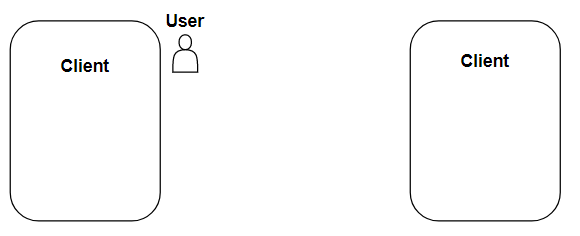
\includegraphics{OAuthFlow1} 
	\caption[Visueel de drie componenten]{Hier zijn visueel de drie componenten van OAuth afgebeeld.}
	\label{fig:oauth1}
\end{figure}
De flow kan uitgelegd worden aan de hand van een voorbeeld. In dit voorbeeld wordt als client een webapplicatie genomen. De api wordt dan voorgesteld als de authorization en resource server van de applicatie waar de webapplicatie de gebruikergegevens van wenst. Om het gemakkelijk te houden zal dit hier Facebook zijn. Merk wel op dat de authorization server niks van persoonlijke informatie over de gebruiker heeft, deze is puur voor authorization. De persoonlijke gegevens en resources van de gebruiker zijn allemaal te vinden op de resource server. Voor de user wordt de naam Jan gebruikt. Dit voorbeeld wordt visueel afgebeeld op figuur \ref{fig:oauth2} \autocite{Deniss2016} \autocite{Services2016}.
\begin{figure}[H]
	\centering
	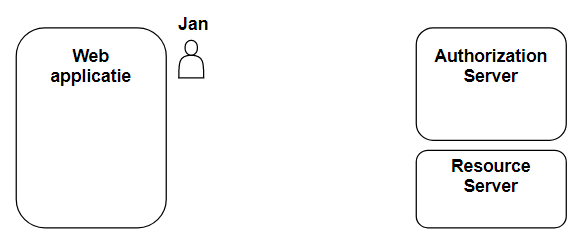
\includegraphics{OAuthFlow2} 
	\caption[De drie componenten aan de hand van een voorbeeld]{Hier zijn visueel de drie componenten van OAuth afgebeeld aan de hand van een voorbeeld.}
	\label{fig:oauth2}
\end{figure}
In dit voorbeeld wenst de gebruiker Jan zijn contacten van Facebook te synchroniseren met zijn contacten op de webapplicatie. Hiervoor heeft de webapplicatie dus de gegevens van Jan nodig die op de resource server van Facebook staan, maar dit zonder het wachtwoord van Jan te weten. Hoe gaat dit in zijn werk?
De eerste stap is dat Jan vraagt om zijn contacten te sychroniseren door op een knop op de webapplicatie te klikken. Wanneer hierop geklikt wordt begint OAuth met het uitvoeren van de flow. De webapplicatie zal een aanvraag sturen naar de authorization server van Facebook en de server zal een inlog scherm tonen aan de gebruiker. Jan kan nu inloggen met zijn gegevens van Facebook op de authorization server. Dit zie je visueel op figuur \ref{fig:oauth3} \autocite{Services2016} \autocite{OktaDev2018}.
\begin{figure}[H]
	\centering
	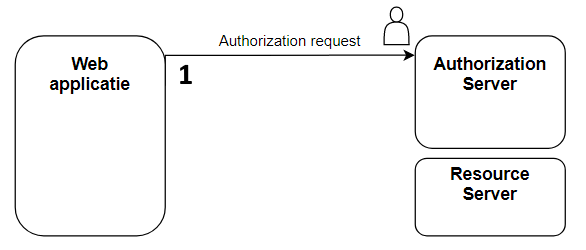
\includegraphics{OAuthFlow3} 
	\caption[Eerste call naar de authorization server]{Hier wordt visueel de eerste call naar de authorization server afgebeeld.}
	\label{fig:oauth3}
\end{figure}
Wanneer Jan heeft ingelogd op de authorization server en een eventueel extra toestemmingsscherm aanvaard heeft, zal de server een authorization grant, waar zich een authorization code in bevindt, terugsturen naar de webapplicatie. Dit is afgebeeld op figuur \ref{fig:oauth4}  \autocite{Services2016}.
\begin{figure}[H]
	\centering
	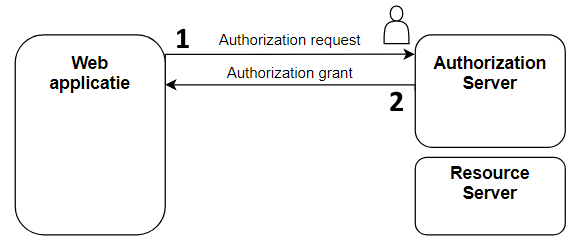
\includegraphics{OAuthFlow4} 
	\caption[Authorization grant wordt teruggestuurd]{Hier wordt visueel afgbeeld dat de authorization server een authorization grant terugstuurd naar de webapplicatie.}
	\label{fig:oauth4}
\end{figure}
De webapplicatie gaat nu deze authorization grant die de authorization code bevat naar de authorization server sturen om zo aan een access token te komen. Deze access token is in de vorm van een bearer token. Deze token zal later gebruikt worden om aan de gegevens van Jan op de resource server te kunnen. Wanneer de authorization server de authorization grant en code van Jan goedkeurt zal deze een access token terugsturen naar de webapplicatie (figuur \ref{fig:oauth5})  \autocite{Services2016} \autocite{OktaDev2018}.
\begin{figure}[H]
	\centering
	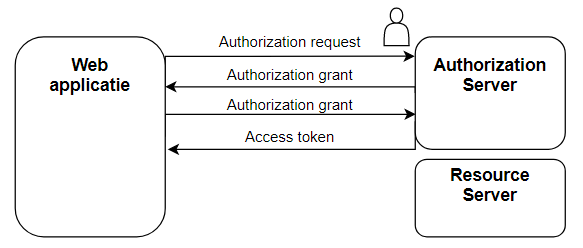
\includegraphics{OAuthFlow5} 
	\caption[Ophalen van de access code]{Hier wordt afgebeeld hoe de webapplicatie die authorization grant terugstuurt naar de authorization server om zo een access code te bemachtigen.}
	\label{fig:oauth5}
\end{figure}
Nu er een geldige access token bemachtigd is, heeft de webapplicatie toegang tot de resource server om zo aan de gegevens van Jan te kunnen. Natuurlijk is het niet de bedoeling dat de webapplicatie zomaar aan alle gegevens van Jan kan. Om dit te vermijden is er nog een belangrijke term binnen OAuth, namelijk scopes. Een authorization request is altijd scoped. Dit betekent in dit voorbeeld dat de authorization request scoped was om enkel de contacten van Jan te bekijken. De webapplicatie kan dus enkel de contacten raadplegen en geen andere persoonlijke informatie van Jan \autocite{Services2016} \autocite{OktaDev2018}. 

Om nu dus aan de contacten van Jan te komen, gaat de webapplicatie dit verzoek naar de resource server sturen met de access token inbegrepen. De resource sever gaat dan kijken of de access token correct is en zo de contacten gaan ophalen en terugsturen naar de webapplicatie (figuur \ref{fig:oauth6}) \autocite{Services2016} \autocite{OktaDev2018}.

\begin{figure}[H]
	\centering
	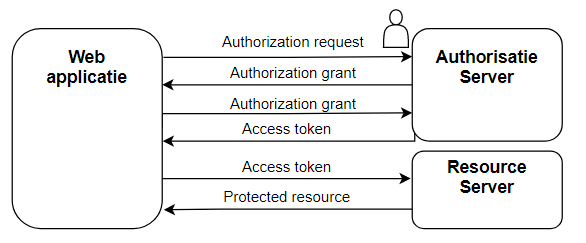
\includegraphics{OAuthFlow6} 
	\caption[Gebruik van access token voor ophalen protected resource]{Hier wordt afgebeeld hoe de webapplicatie met de access token de protected resources van de user gaat ophalen.}
	\label{fig:oauth6}
\end{figure}
Merk op dat OAuth hier dient als het authorization framework. De authentication van de gebruiker Jan gebeurt met openId connect door het gebruik van id-tokens die mee gegeven worden met de access token \autocite{OktaDev2018}.

Om dit allemaal te laten werken is er een belangrijke stap die niet vergeten mag worden. Voordat de webapplicatie deze flow kan hanteren met een api, in dit geval Facebook, moet de webapplicatie zich eerst registreren bij de Facbook api service. Om dit te doen moet de webapplicatie zijn naam, website en callback url opgeven. Een callback url is simpelweg een url naar waar de api zal redirecten na het identificeren van de gebruiker. Wanneer de webapplicatie deze gegevens aan de api service gegeven heeft, krijgt deze een clientId en een client secret terug. Een cleintId is een publieke en unieke key die gebruikt wordt om de webapplicatie te identificeren als applicatie. De client secret is een private key die geheimgehouden wordt tussen de applicatie en de api. Deze secret wordt gebruikt om de applicatie te identificeren wanneer deze een verzoek doet voor een access token \autocite{OktaDev2018}. 

\subsection{\IfLanguageName{dutch}{Grant types van OAuth}{Grant types of OAuth}}
Om de vier verschillende grant types van OAuth te bekijken is het belangrijk bovenstaand voorbeeld meer in detail te bekijken (figuur \ref{fig:grantTypes1}).
\begin{figure}[H]
	\centering
	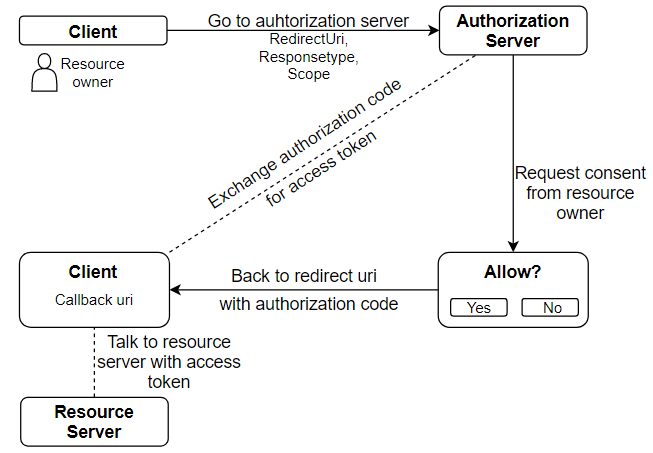
\includegraphics{GrantTypes1} 
	\caption[Gedetailleerd voorbeeld voor uitleg grant types]{Dit is het voorgaande voorbeeld gedetailleerd uitgewerkt.}
	\label{fig:grantTypes1}
\end{figure}
In deze figuur is dezelfde flow als het vorige voorbeeld uitgetekend. Het is belangrijk dit zo uit te tekenen voordat er verder wordt ingegaan op grant types.
Het eerste wat besproken moet worden is netwerkcommunicatie. Binnen netwerkcommunicatie zijn er twee mogelijke channels die gebruikt kunnen worden voor communicatie. Deze worden opgesplits in \autocite{OktaDev2018}: 
\begin{itemize}
	\item Back channel (highly secured)
	\item Front channel (less secured channel)
\end{itemize}
\subsubsection{\IfLanguageName{dutch}{Back channel (highly secured)}{Back channel (highly secured)}}
Een back channel is de veiligste channel van de twee om gegevens uit te wisselen. Deze uitwisseling gebeurt vaak over https, is vaak SSL encrypted en kan niet onderschept worden. Deze channel wordt vaak gebruikt voor communicatie tussen twee servers of api's \autocite{OktaDev2018}.
\subsubsection{\IfLanguageName{dutch}{Front channel (less secured channel)}{Front channel (less secured channel)}}
Front channel is minder beveiligd dan een back channel. Een goed voorbeeld van front channel communicatie is bijvoorbeeld de browser. Deze is veilig, maar als er gekeken wordt naar hoe een browser gebouwd is, valt op dat er loopholes of datalekken kunnen zijn. Alles wat met front channel verstuurd wordt, kan mogelijks zelfs gewoon in de url afgelezen worden \autocite{OktaDev2018}.
\subsubsection{\IfLanguageName{dutch}{Grant types}{Grant types}}
Bij het bekijken van figuur \ref{fig:grantTypes1} kan je een verschil zien tussen stippellijnen en volle lijnen. Deze staan voor welke channel er gebruikt wordt. Aangezien front channel minder beveiligd is dan back channel wordt deze gebruikt voor alles wat niet super beveiligd moet worden, zoals het uitwisselen van de authorization grant. Als dit onderschept zou worden, zou het niet zo erg zijn, met een authorization grant is een potentiele hacker niks \autocite{OktaDev2018}. 

Wat wel beveiligd moet worden, is de access token en mogelijke id-token. Als deze onderschept wordt door een potentiele hacker, kan deze aan de persoonlijke gegevens van de gebruiker op de resource server. Daarom wordt hiervoor de back channel gebruikt. Dit is ook meteen de reden waarom er tweemaal terug wordt gegaan naar de authorization server in plaats van dat deze in één keer de access token meestuurt in de front channel \autocite{OktaDev2018}.

Nu de verschillende channels zijn uitgeklaard kunnen de vier grant types van OAuth besproken worden. De vier grant types van OAuth zijn de volgende \autocite{OktaDev2018}:
\begin{itemize}
	\item Authorization code grant (front + back channel)
	\item Implicit (alleen front channel)
	\item Resource owner password credentials (alleen back channel)
	\item Client credentials (alleen back channel)
\end{itemize}
In \ref{fig:grantTypes1} zie je een voorbeeld van authorization code grant. Dit is de grant type die het meest gebruikt wordt bij webapplicaties met een server backend. Deze grant type is ook meteen de veiligste aangezien deze gebruik maakt van zowel front- als back channelcommunicatie \autocite{OktaDev2018}.

De op een na meest gebruikte grant type is implicit flow. Deze grant type is iets minder veilig dan authorization code grant, maar wordt vaak gebruikt bij bijvoorbeeld javascript applicaties \autocite{OktaDev2018}. 

Aangezien authorization code grant en implicit flow de meest gebruikte zijn zie je in figuur \ref{fig:grantTypes2} ook een visueel voorbeeld van een implicit flow. Nu is het mogelijk om duidelijk het verschil te zien in de flow.
\begin{figure}[H]
	\centering
	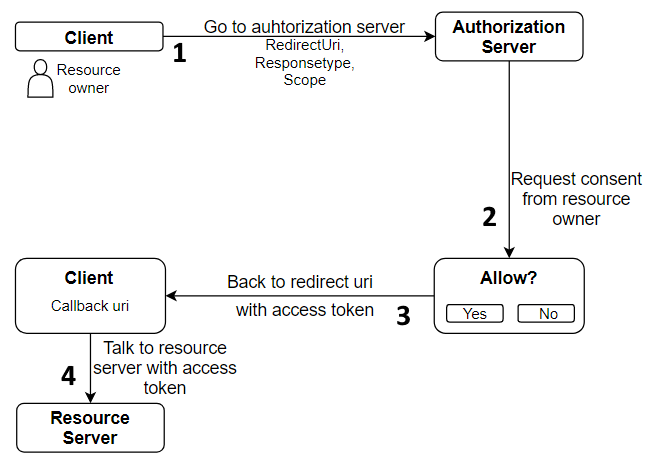
\includegraphics{GrantTypes2} 
	\caption[Visuele voorstelling van implicit grant]{Hier zie je het zelfde schema als de vorige voorbeelden, maar dan met implicit grant in plaats van authorization code grant.}
	\label{fig:grantTypes2}
\end{figure}
Zoals je kan zien in figuur \ref{fig:grantTypes2} zijn nu alle requests met volle lijnen in plaats van met stippellijnen. Dit komt dus omdat er bij implicit flow geen back channel communicatie gebruikt wordt. Hier gebeurt alles met front channel communicatie. Wat ook opvalt is dat hier meteen de access token door de authorization server wordt meegestuurd in plaats van eerst een authorization grant met authorization code. Er moest dus één request minder naar de authorization server gedaan worden. Het nadeel van deze flow is dus wel dat het minder veilig is dan authorization code grant \autocite{OktaDev2018}. 

Bij authorization code grant worden het uitwisselen van access token met de authorization server en alle communicatie met de resource server dus via de back channel gedaan. Dit is dus omdat deze access token niet in de verkeerde handen mag vallen. Bij elk request naar de resource server wordt deze access token ook mee gestuurd en daarom gebeuren deze requests ook via de back channel \autocite{OktaDev2018}.

De client credentials flow en resource owner password credentials worden minder gebruikt. Client credentials flow wordt soms nog gebruikt bij machine-naar-machinecommunicatie en resource owner password credentials wordt soms nog gebruikt om oudere applicaties juist te doen werken. Beide zijn ze echter niet meer aan te raden om te gebruiken \autocite{OktaDev2018}.

\subsection{\IfLanguageName{dutch}{Authentication vs authorization}{Authentication vs authorization}}
Zoals eerder vermeld is het OAuth-framework enkel bedoeld voor authorization, maar met enkele aanpassingen kan het ook gebruikt worden voor authentication. Maar wat is nu precies het verschil \autocite{rwike772020}?

Authentication is het proces van bewijzen dat je bent wie je zegt dat je bent. Dit is dus niet te vergelijken met authorization, dat dient om een geïdentificeerde partij toestemming te geven om iets te doen en om te bepalen tot welke gegevens deze partij toegang heeft \autocite{rwike772020}.

\subsection{\IfLanguageName{dutch}{OpenId connect}{OpenId connect}}
Als OAuth enkel bedoeld is voor authorization, wat is die id-token dan en hoe doe je aan authentication? Zoals gezegd kan je met een kleine aanpassing zorgen dat je met OAuth ook aan authentication kan doen. Dit framework heet openId connect. \autocite{rwike772019} \autocite{rwike772019a}

Toen openId connect nog niet bestond werd OAuth ook al door velen gebruikt, maar niet zoals het hoorde. Veel mensen vonden de authorization mogelijkheden van OAuth zo makkelijk dat ze dit graag wilden gebruiken, maar ze wilden er ook graag authentication mee doen. Door dit te forceren werd het framework fout gebruikt en ontstonden er verschillende implementaties die niet op elkaar afgestemd waren en dit zorgde voor onduidelijkheid \autocite{rwike772019} \autocite{rwike772019a}.

Hierdoor ontstond openId connect. Dit is een framework gebouwd boven op het OAuth-framework waardoor authentication mogelijk is. OpenId connect is het framework dat ervoor zorgt dat er niet enkel een access token wordt gestuurd van de authorisation server naar de client, maar ook een id-token. Hiermee kan de user dan geverifieerd worden \autocite{rwike772019} \autocite{rwike772019a}.

\section{\IfLanguageName{dutch}{Geschiedenis van OAuth}{History of OAuth}}
\label{sec:OAuthHistory}
In 2007 is de OAuth-discussiegroep gestart als een samenwerkingsinitiatief om toegang tot beschermde bronnen van gebruikers mogelijk te maken zonder dat hun inloggegevens bekend hoeven te worden gemaakt. De eerste versie van het OAuth-framework (OAuth 1.0) is opgesteld in oktober 2007 en in april 2010 uitgebracht als een RFC (request for comments) \autocite{Chen2014}.

Het framework heeft sindsdien verschillende herzieningen ondergaan. De belangrijkste verbeteringen van het protocol zijn in oktober 2012 uitgebracht als het OAuth 2.0 framework \autocite{Chen2014}.

\subsection{\IfLanguageName{dutch}{OAuth 1.0}{OAuth 1.0}}
Toen de eerste versie van OAuth werd opgesteld, was er nog een ander algemeen authenticatie framework, genaamd openID (niet te verwarren met openId connect). Daarom is OAuth speciaal ontwikkeld om een probleem op te lossen dat niet onder openID valt: een stabiele overdracht van toegang tot de api. Hoewel soms de term api-authenticatie werd gebruikt om de OAuth-functies te karakteriseren, was het framework zelf nooit bedoeld voor gebruikersauthenticatie \autocite{Chen2014}.

Twee jaar na de release van het concept OAuth 1.0 werd een aanval ontdekt tegen de goedkeuringsfase van de access token van het framework. Er is een wijziging van het oorspronkelijke framework (genaamd OAuth 1.0a) uitgebracht om de bug te corrigeren \autocite{Chen2014}.
\subsection{\IfLanguageName{dutch}{OAuth 2.0}{OAuth 2.0}}
OAuth 1.0 (en OAuth 1.0a) hadden enkele belangrijke nadelen aan hun gebruiksscenario's. In plaats van het huidige protocol uit te breiden, stemde de werkgroep ermee in de specificatie volledig te wijzigen om een nieuw OAuth 2.0 framework te creëren. Volgens een vertrekkende hoofdauteur van OAuth 1.0 was deze beslissing het resultaat van een ernstig en onoverbrugbaar conflict tussen verschillende belangengroepen \autocite{Chen2014}.

Een grote verandering was de toevoeging van bearertokens die door OAuth 2.0 werden geïmplementeerd. Dat wil zeggen, de access token van een gebruiker was niet langer gebonden aan een vertrouwde client, maar elke client die in het bezit is van deze token heeft vrije toegang tot de beschermde resource van de gebruiker. OAuth 2.0 biedt ook vier methoden voor het uitwisselen van access tokens. Deze methoden worden grants genoemd en kunnen worden gezien als afzonderlijke "modellen" van OAuth 2.0. De verschillende grants zijn reeds besproken \autocite{Chen2014}.
\section{\IfLanguageName{dutch}{Microsoft azure active directory}{Microsoft azure active directory}}
\label{sec:AzureRollingKeys}
Azure Active Directory (Azure AD) is de cloudgebaseerde service voor identiteits- en toegangsbeheer die wordt aangeboden door Microsoft. Hiermee kunnen werknemers zich aanmelden en toegang hebben tot external resources zoals Microsoft Office 365, Azure portal, en duizenden andere SaaS applicaties, maar ook interne resources zoals apps op het bedrijfsnetwerk en intranet, samen met elke cloud app gemaakt door het bedrijf zelf \autocite{Boucher2019} \autocite{msaburnley2019}.
\subsection{\IfLanguageName{dutch}{Rolling keys}{Rolling keys}}
Azure AD maakt gebruik van openbare cryptografie op basis van industriestandaarden om vertrouwen te creëren tussen zichzelf en de applicaties die het gebruiken. In praktische termen werkt dit als volgt: Azure AD gebruikt een signing key die bestaat uit een combinatie van public en private key. Azure AD produceert een security token die informatie over de gebruiker bevat wanneer een gebruiker zich aanmeldt bij een toepassing die Azure AD gebruikt voor verificatie. Azure AD gebruikt zijn private key om deze token te ondertekenen voordat de key wordt teruggestuurd naar de server. Om te verifiëren dat de token legitiem is en afkomstig is van Azure AD, moet de toepassing de handtekening van de token valideren met behulp van de public Azure AD key in het OpenID Link discovery document  \autocite{Boucher2019} \autocite{msaburnley2019}.

De signing key van Azure AD rolt regelmatig om veiligheidsredenen en kan in geval van nood automatisch worden omgedraaid. Elk programma dat is geïntegreerd met Azure AD moet in staat zijn om een main rollover event aan te kunnen, ongeacht hoe vaak dit kan gebeuren. Als dit niet het geval is, en je applicatie wil een verlopen sleutel gebruiken om de handtekening op een token te controleren, dan zal het inloggen mislukken  \autocite{Boucher2019} \autocite{msaburnley2019} \autocite{rwike772018}.

Het OpenID Link discovery document bevat vaak meer dan één geldige sleutel. Je applicatie moet bereid zijn om alle sleutels te gebruiken die in het document worden vermeld, aangezien één sleutel binnenkort kan worden gerold, een andere sleutel aan vervanging toe kan zijn  \autocite{Boucher2019} \autocite{msaburnley2019}.

%%=============================================================================
%% Methodologie
%%=============================================================================

\chapter{\IfLanguageName{dutch}{Methodologie}{Methodology}}
\label{ch:methodologie}

%% TODO: Hoe ben je te werk gegaan? Verdeel je onderzoek in grote fasen, en
%% licht in elke fase toe welke stappen je gevolgd hebt. Verantwoord waarom je
%% op deze manier te werk gegaan bent. Je moet kunnen aantonen dat je de best
%% mogelijke manier toegepast hebt om een antwoord te vinden op de
%% onderzoeksvraag.

\lipsum[21-25]



% Voeg hier je eigen hoofdstukken toe die de ``corpus'' van je bachelorproef
% vormen. De structuur en titels hangen af van je eigen onderzoek. Je kan bv.
% elke fase in je onderzoek in een apart hoofdstuk bespreken.

%\input{...}
%\input{...}
%...

%%=============================================================================
%% Conclusie
%%=============================================================================

\chapter{Conclusie}
\label{ch:conclusie}

% TODO: Trek een duidelijke conclusie, in de vorm van een antwoord op de
% onderzoeksvra(a)g(en). Wat was jouw bijdrage aan het onderzoeksdomein en
% hoe biedt dit meerwaarde aan het vakgebied/doelgroep? 
% Reflecteer kritisch over het resultaat. In Engelse teksten wordt deze sectie
% ``Discussion'' genoemd. Had je deze uitkomst verwacht? Zijn er zaken die nog
% niet duidelijk zijn?
% Heeft het onderzoek geleid tot nieuwe vragen die uitnodigen tot verder 
%onderzoek?

In dit onderzoek werd zowel een antwoord gegeven op de onderzoeksvraag alsook op verschillende deelvragen. De onderzoeksvraag was: \emph{Hoe kan Ventigrate op een professionele manier APIs en clients opzetten beveiligd door Azure active directory aan de hand van rolling keys?}. \newline \newline 
Uit dit onderzoek werd geleerd hoe JWT bearer authenticatie in zijn werk gaat. Hieruit werd geconcludeerd dat een JWT token of JSON web token bestaat uit drie delen, een header, payload en signature. Wat opviel is dat de header vier claims bevat die essentieel zijn voor het valideren van de token. De payload bevat meer claims maar niet allemaal verplicht. Tot deze claims behoren bijvoorbeeld de audiance of de roles maar die kan ook de openId claim bevatten wanneer er ook aan authenticatie gedaan wordt. Het signature deel kan worden gebruikt om de authenticiteit van het token te valideren, zodat het door de applicatie kan worden vertrouwd. \newline \newline
Op de deelvragen hoe je een API moet beveiligen met client credential of implicit grant wordt antwoord gegeven op een schematische wijze. Aan de hand van enkele stappen wordt een schema opgebouwd om zo de onderliggende werking te verduidelijken. Uit beide onderzoeken zijn gelijkaardige resultaten gevonden. Op het gebruik van de access token na verloopt de flow tussen Azure active directory, api en client gelijkaardig. In beide onderzoeken wordt vooral aandacht besteed aan de verschillende termen en gegevens die terug te vinden zijn bij het doorlopen van de stappen, zoals bijvoorbeeld client ID, resource ID en client secret. Het gebruik van deze waarden moet discreet en juist gebeuren. Er wordt in beide gevallen ook verwezen naar een gemaakte proof of concept als voorbeeld. Deze is echter enkel bedoeld voor demonstratiedoeleinden en is zeker niet aan te raden voor development. De reden hiervoor is dat de discrete waarden zoals, client secret, opgeslagen worden in een json-file in de applicatie. Wanneer we deze proof of concept in development zouden gebruiken, zouden we deze opslaan in een key vault of user secret.\newline\newline
Wanneer wordt gekeken naar hoe een API kan aangesproken worden met authorization code grant valt op dat de schematische voorstelling gelijkaardig is aan de voorgaande voorbeelden. Het verschil dat hier opvalt is de extra call naar AAD voor een athorize code.\newline\newline
Bij Azure key rollover is het belangrijk om te weten welk type situatie je hebt. Bij dit onderzoek zien we dat er verschillende situaties zijn waar clients anders reageren op een key rollover van Azure. In de voorbeelden die bij de vorige deelvragen gebruikt werden hadden we te maken met een clientapplicatie die toegang heeft tot een resource en een webapplicatie die gebruik maakte van JWT Bearer authentication. In de eerste situatie moet er geen rekening gehouden worden met key rollovers aangezien ze geen resources beschermen en hierdoor inspecteren ze de token niet. Bij JWT Bearer token authentication wordt de logica om een key rollover te verwerken al toegevoegd.\newline\newline
Kortom, de onderzoeksvraag kan worden beantwoord aan de hand van de verschillende antwoorden op de deelvragen. Ventigrate kan op een professionele manier APIs en clients opzetten en beveiligen met Azure active directory aan de hand van rolling keys door aan de hand van wat gewenst is het antwoord van de juiste situatie te implementeren. Terwijl dit gebeurt zal de lezer het onderwerp ook beter begrijpen en weten wat er zich achter de schermen afspeelt.



%%=============================================================================
%% Bijlagen
%%=============================================================================

\appendix
\renewcommand{\chaptername}{Appendix}

%%---------- Onderzoeksvoorstel -----------------------------------------------

\chapter{Onderzoeksvoorstel}

Het onderwerp van deze bachelorproef is gebaseerd op een onderzoeksvoorstel dat vooraf werd beoordeeld door de promotor. Dat voorstel is opgenomen in deze bijlage.

% Verwijzing naar het bestand met de inhoud van het onderzoeksvoorstel
%---------- Inleiding ---------------------------------------------------------

\section{Introductie} % The \section*{} command stops section numbering
\label{sec:introductie}

Het framework OAuth 2.0 is een autorisatie framework dat gebruik maakt van keys. OAuth 2.0 wordt gebruikt als een manier voor gebruikers om applicaties toegang te geven tot hun informatie van een betrouwde applicatie, maar zonder hun wachtwoord rechtstreeks op de onbekende applicatie in te geven. In plaats hiervan wordt het wachtwoord op de oauth server ingegeven. Voordat OAuth in omgang was maakten services gebruik van de effectieve wachtwoorden van de gebruiker en niet de key die van de oauth server teruggestuurd wordt om zo aan de gegevens van de gebruiker te kunnen. Er was geen zekerheid wat er hierna met het wachtwoord gebeurde, hierdoor is OAuth in het leven geroepen. Dit framework wordt gebruikt door bedrijven zoals Google, Facebook, Microsoft en Twitter om de gebruikers in staat te stellen informatie over hun accounts te delen met applicaties van derden.\newline\newline
In dit onderzoek ga ik op zoek naar de verschillende validatiemogelijkheden van OAuth 2.0 aan de hand van rolling keys, vergelijk ik die met alternatieven en zijn voorganger OAuth en bespreek ik de implementatie in de bedrijfswereld.

%---------- Stand van zaken ---------------------------------------------------

\section{Stand van zaken}
\label{sec:state-of-the-art}

Bij grotere bedrijven wordt dit framework al enkele jaren gebruikt en blijft het ook gebruikt worden door de eenvoud en veiligheid. Kleinere bedrijven gaan ook steeds meer aan de slag met OAuth 2.0 en er is ook veel vraag naar binnen development. Op het internet is er ook veel uitleg over het OAuth 2.0 framework, maar dan vooral over de technische werking (\cite{Deniss2016}). \newline\newline
Dit is dus een onderwerp waar nog veel over onderzocht kan worden en waar veel belangrijke randinformatie over te vinden valt. Enkele huidige OAuth service providers zijn Amazon, Apple, Facebook, Github en nog enkelen.

% Voor literatuurverwijzingen zijn er twee belangrijke commando's:
% \autocite{KEY} => (Auteur, jaartal) Gebruik dit als de naam van de auteur
%   geen onderdeel is van de zin.
% \textcite{KEY} => Auteur (jaartal)  Gebruik dit als de auteursnaam wel een
%   functie heeft in de zin (bv. ``Uit onderzoek door Doll & Hill (1954) bleek
%   ...'')


%---------- Methodologie ------------------------------------------------------
\section{Methodologie}
\label{sec:methodologie}

Om de volledige werking van OAuth 2.0 te onderzoeken, zal ik mij baseren op reeds bestaande literatuur over de veiligheid en werking van het framework. In een paper van Erik Chen is te lezen hoe het protocol al verschillende malen herwerkt is de voorbije jaren en ook dat het verschillend is voor webapplicaties en mobiele applicaties (\cite{Chen2014}). \newline 
Met deze informatie zal ik afwegen welke validatiemogelijkheden er bestaan met OAuth 2.0. Van deze informatie zal ik dan gebruik maken om het OAuth 2.0 framework te gebruiken in een applicatie om mij zo nog meer te verdiepen in de werking en mogelijkheden. Al deze resultaten zal ik met elkaar gaan vergelijken om zo de validatiemogelijkheden en voor-/nadelen van het framework te achterhalen.

%---------- Verwachte resultaten ----------------------------------------------
\section{Verwachte resultaten}
\label{sec:verwachte_resultaten}

Ik verwacht de werking van het OAuth 2.0 framework te doorgronden en zo de voordelen van de eenvoud en veiligheid te kunnen documenteren en dit framework te vergelijken met andere authenticatieframeworks of voorgangers van het framework. Ik verwacht ook dat ik enkele fouten van het framework zal tegenkomen. Zo lees je in de papers van Pili Hu en Eugene Ferry dat er de voorbije jaren al veel aanvallen, loopholes en fouten zijn ontdekt in het framework. Deze zou ik ook gaan onderzoeken. Ik wil kijken waar er al wel of niet verbeteringen aangebracht zijn (\cite{Hu2014}) (\cite{Ferry2015}). \newline
Door deze vergelijkingen te maken, hoop ik de mogelijkheden en voor-/nadelen van het framework te vinden en deze te kunnen documenteren en aan te tonen. 

%---------- Verwachte conclusies ----------------------------------------------
\section{Verwachte conclusies}	
\label{sec:verwachte_conclusies}

Na het onderzoek en een proof of concept te maken hoop ik met mijn kennis over het OAuth 2.0 framwork een document te kunnen samenstellen waar ik de voordelen en eventuele nadelen over het OAuth 2.0 framework bespreek. Zo zou ik het graag hebben over de veiligheid, eenvoud en werking van OAuth 2.0. Hier wil ik mee bereiken dat bedrijven aan de hand van dit document kunnen beslissen of ze het OAuth 2.0 framework zullen opnemen in toekomstige projecten bij hun klanten.




%%---------- Andere bijlagen --------------------------------------------------
% TODO: Voeg hier eventuele andere bijlagen toe
%\input{...}

%%---------- Referentielijst --------------------------------------------------

\printbibliography[heading=bibintoc]

\end{document}
